\documentclass[tikz,border=12pt]{standalone}
\usepackage[T1]{fontenc}
\usepackage{mathpazo}
\usepackage{amsmath,amssymb}
\usetikzlibrary{arrows.meta, positioning, calc, shadows.blur}

\definecolor{stblue}{HTML}{7B97AD}
\definecolor{sage}{HTML}{7A9A7E}
\definecolor{rwgold}{HTML}{B8995E}
\definecolor{terracotta}{HTML}{C47A6A}
\definecolor{lavender}{HTML}{907EA0}
\definecolor{dkbrown}{HTML}{3D3530}
\definecolor{wmgray}{HTML}{7B7067}
\definecolor{cream}{HTML}{F9F6F0}
\definecolor{border}{HTML}{D4C9B8}

\begin{document}
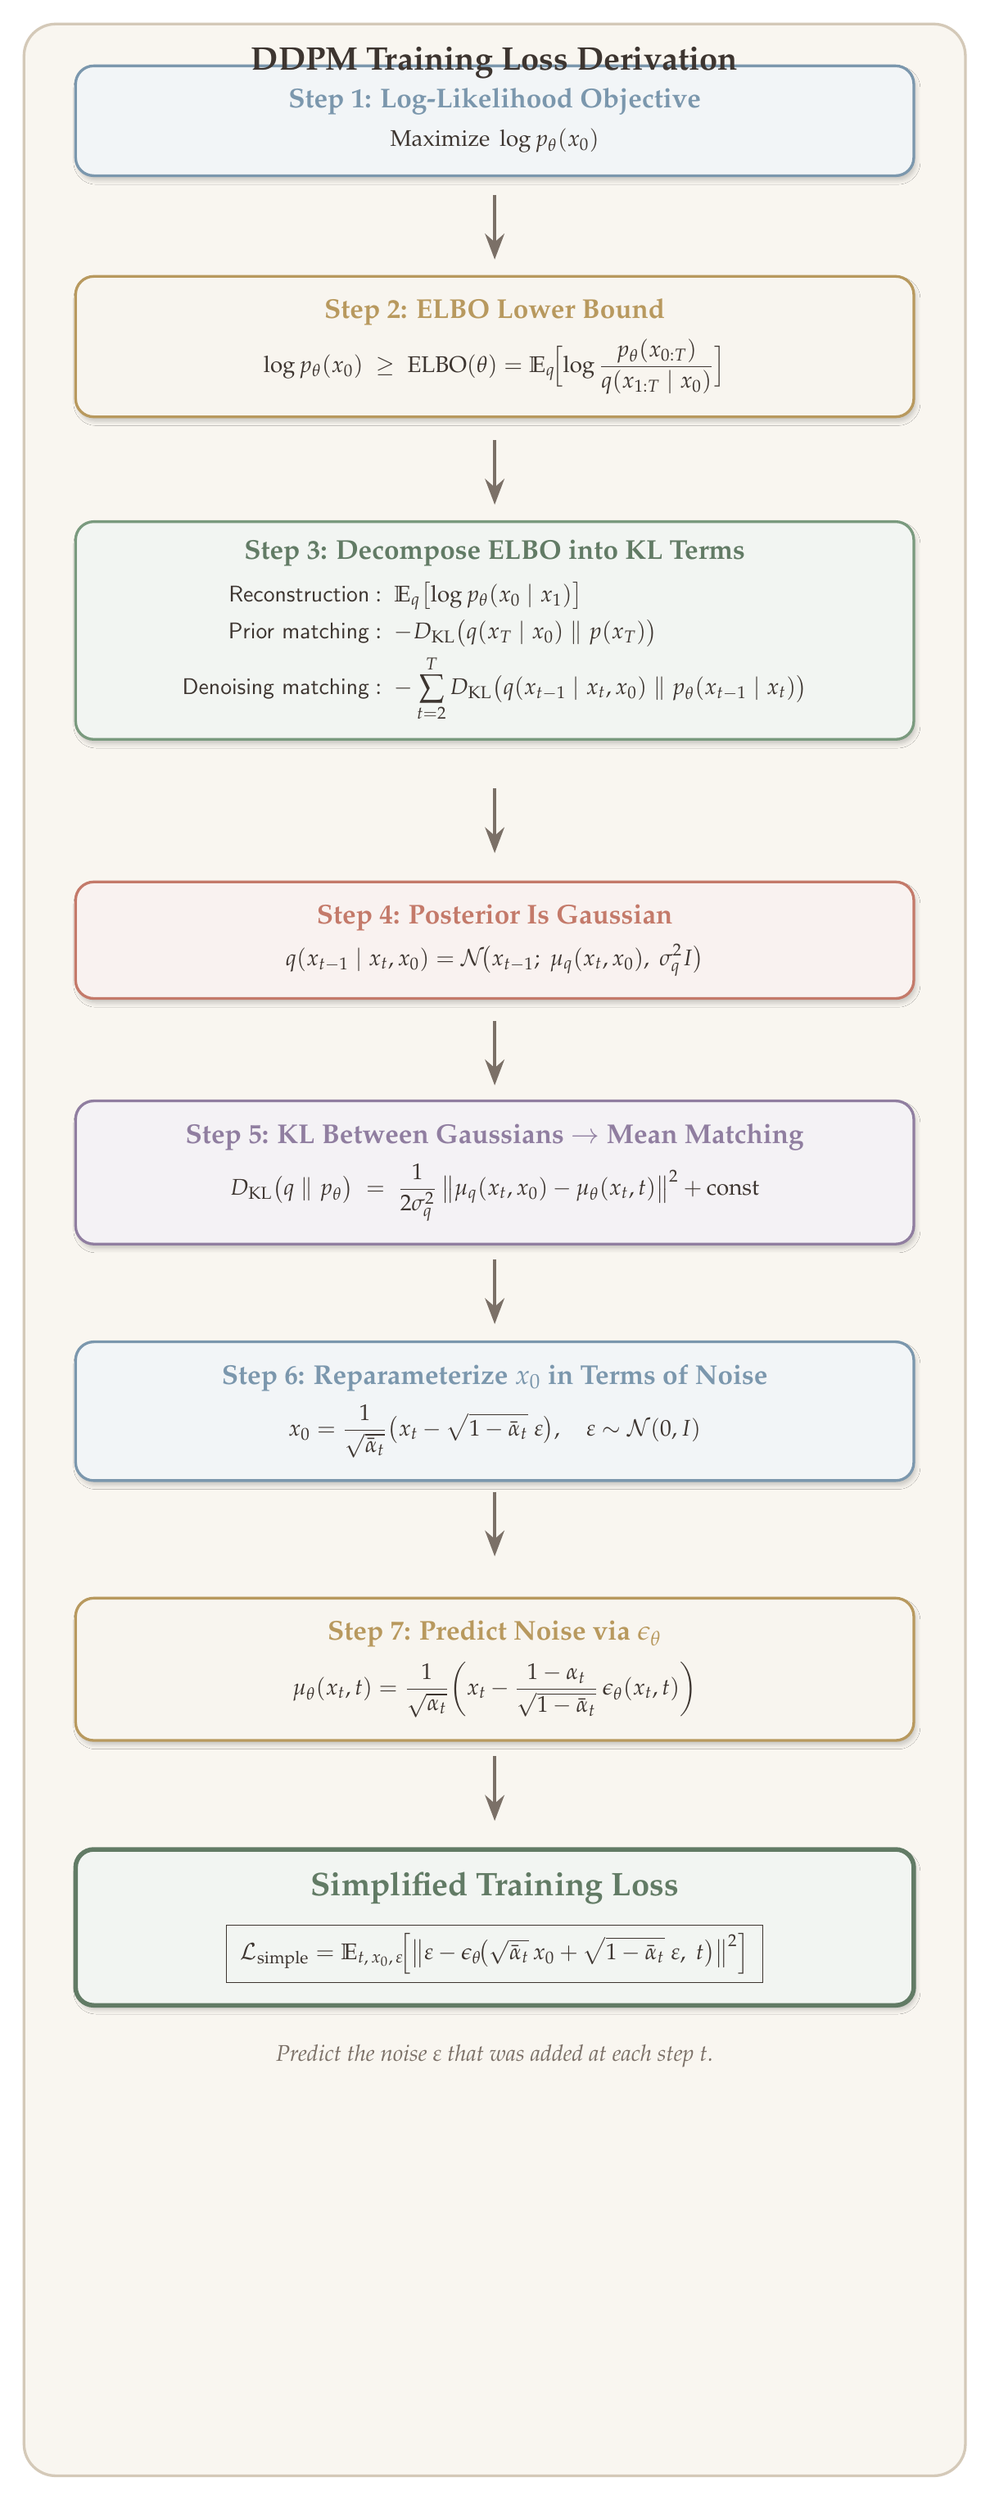
\begin{tikzpicture}[>={Stealth[length=4mm, width=3mm]}, line width=1.5pt,
  stepbox/.style 2 args={
    draw=#1, line width=1.2pt, fill=#1!10, rounded corners=8pt,
    minimum width=13cm, align=center, inner sep=10pt,
    text=dkbrown,
    blur shadow={shadow blur steps=5, shadow xshift=1pt, shadow yshift=-2pt,
                 shadow opacity=20}
  }]

% Background
\fill[cream, rounded corners=14pt] (-7.3,-1.0) rectangle (7.3,37.0);
\draw[border, line width=1.2pt, rounded corners=14pt] (-7.3,-1.0) rectangle (7.3,37.0);

% --- Step 1: Log-likelihood ---
\node[stepbox={stblue}{}] (s1) at (0,35.5)
  {{\large\bfseries\color{stblue} Step 1: Log-Likelihood Objective}\\[5pt]
   $\displaystyle \text{Maximize } \log p_\theta(x_0)$};

% Arrow
\draw[wmgray, ->, line width=1.5pt] (0,34.35) -- (0,33.35);

% --- Step 2: ELBO ---
\node[stepbox={rwgold}{}] (s2) at (0,32.0)
  {{\large\bfseries\color{rwgold} Step 2: ELBO Lower Bound}\\[5pt]
   $\displaystyle \log p_\theta(x_0) \;\geq\; \text{ELBO}(\theta)
    = \mathbb{E}_q\!\Bigl[\log \frac{p_\theta(x_{0:T})}{q(x_{1:T}\mid x_0)}\Bigr]$};

% Arrow
\draw[wmgray, ->, line width=1.5pt] (0,30.55) -- (0,29.55);

% --- Step 3: Decompose ELBO ---
\node[stepbox={sage}{}, inner sep=8pt] (s3) at (0,27.6)
  {{\large\bfseries\color{sage!80!black} Step 3: Decompose ELBO into KL Terms}\\[6pt]
   \begin{tabular}{@{}r@{\;:\;\;}l@{}}
     \textsf{Reconstruction} &
       $\mathbb{E}_q\bigl[\log p_\theta(x_0 \mid x_1)\bigr]$ \\[4pt]
     \textsf{Prior matching} &
       $-D_{\mathrm{KL}}\bigl(q(x_T \mid x_0)\;\|\;p(x_T)\bigr)$ \\[4pt]
     \textsf{Denoising matching} &
       $-\displaystyle\sum_{t=2}^{T}
         D_{\mathrm{KL}}\bigl(q(x_{t-1}\mid x_t, x_0)
         \;\|\; p_\theta(x_{t-1}\mid x_t)\bigr)$
   \end{tabular}};

% Arrow
\draw[wmgray, ->, line width=1.5pt] (0,25.15) -- (0,24.15);

% --- Step 4: Posterior is Gaussian ---
\node[stepbox={terracotta}{}] (s4) at (0,22.8)
  {{\large\bfseries\color{terracotta} Step 4: Posterior Is Gaussian}\\[5pt]
   $\displaystyle q(x_{t-1} \mid x_t, x_0)
    = \mathcal{N}\!\bigl(x_{t-1};\; \mu_q(x_t, x_0),\; \sigma_q^2 I\bigr)$};

% Arrow
\draw[wmgray, ->, line width=1.5pt] (0,21.55) -- (0,20.55);

% --- Step 5: KL -> mean matching ---
\node[stepbox={lavender}{}] (s5) at (0,19.2)
  {{\large\bfseries\color{lavender} Step 5: KL Between Gaussians $\to$ Mean Matching}\\[5pt]
   $\displaystyle D_{\mathrm{KL}}\bigl(q \;\|\; p_\theta\bigr)
    \;=\; \frac{1}{2\sigma_q^2}\,
    \bigl\|\mu_q(x_t, x_0) - \mu_\theta(x_t, t)\bigr\|^2
    + \text{const}$};

% Arrow
\draw[wmgray, ->, line width=1.5pt] (0,17.85) -- (0,16.85);

% --- Step 6: Reparameterize x_0 ---
\node[stepbox={stblue}{}] (s6) at (0,15.5)
  {{\large\bfseries\color{stblue} Step 6: Reparameterize $x_0$ in Terms of Noise}\\[5pt]
   $\displaystyle x_0 = \frac{1}{\sqrt{\bar\alpha_t}}
    \bigl(x_t - \sqrt{1-\bar\alpha_t}\;\varepsilon\bigr),
    \quad \varepsilon \sim \mathcal{N}(0,I)$};

% Arrow
\draw[wmgray, ->, line width=1.5pt] (0,14.25) -- (0,13.25);

% --- Step 7: Noise prediction form ---
\node[stepbox={rwgold}{}] (s7) at (0,11.5)
  {{\large\bfseries\color{rwgold} Step 7: Predict Noise via $\epsilon_\theta$}\\[5pt]
   $\displaystyle \mu_\theta(x_t, t)
    = \frac{1}{\sqrt{\alpha_t}}
    \biggl(x_t - \frac{1-\alpha_t}{\sqrt{1-\bar\alpha_t}}\,
    \epsilon_\theta(x_t, t)\biggr)$};

% Arrow
\draw[wmgray, ->, line width=1.5pt] (0,10.15) -- (0,9.15);

% --- Step 8: Simplified loss ---
\node[stepbox={sage}{}, line width=2pt, draw=sage!80!black] (s8) at (0,7.5)
  {{\Large\bfseries\color{sage!80!black} Simplified Training Loss}\\[8pt]
   $\displaystyle \boxed{\;\mathcal{L}_{\mathrm{simple}}
    = \mathbb{E}_{t,\, x_0,\, \varepsilon}\!
    \Bigl[\bigl\|\varepsilon - \epsilon_\theta\!\bigl(
    \sqrt{\bar\alpha_t}\,x_0 + \sqrt{1-\bar\alpha_t}\;\varepsilon,\; t
    \bigr)\bigr\|^2\Bigr]\;}$};

% Decorative note below final box
\node[text=wmgray, font=\itshape, align=center] at (0,5.5)
  {Predict the noise $\varepsilon$ that was added at each step $t$.};

% Title at the very top (inside background)
\node[text=dkbrown, font=\Large\bfseries] at (0,36.4)
  {DDPM Training Loss Derivation};

\end{tikzpicture}
\end{document}
